%%
%% This is file `mcmthesis-demo.tex',
%% generated with the docstrip utility.
%%
%% The original source files were:
%%
%% mcmthesis.dtx  (with options: `demo')
%% !Mode:: "TeX:UTF-8"
%% -----------------------------------
%%
%% This is a generated file.
%%
%% Copyright (C)
%%     2010 -- 2015 by latexstudio
%%     2014 -- 2016 by Liam Huang
%%     2014 -- 2016 by latexstudio.net
%%
%% This work may be distributed and/or modified under the
%% conditions of the LaTeX Project Public License, either version 1.3
%% of this license or (at your option) any later version.
%% The latest version of this license is in
%%   http://www.latex-project.org/lppl.txt
%% and version 1.3 or later is part of all distributions of LaTeX
%% version 2005/12/01 or later.
%%
%% This work has the LPPL maintenance status `maintained'.
%%
%% The Current Maintainer of this work is Liam Huang.
%%
\documentclass{mcmthesis}
\mcmsetup{CTeX = true,   % 使用 CTeX 套装时,设置为 true
        tcn =2021953, problem = D,
        sheet = true, titleinsheet = true, keywordsinsheet = true,
        titlepage = true, abstract = true}
\usepackage{palatino}
\usepackage{lipsum}
\usepackage{graphicx}
\usepackage{float}
\usepackage{booktabs}
\usepackage{verbatim}
\usepackage{cite}
\newcommand{\upcite}[1]{\textsuperscript{\textsuperscript{\cite{#1}}}}
\usepackage{listings}
\usepackage{xcolor} %代码高亮
 
\lstset{numbers=left, %设置行号位置
        numberstyle=\footnotesize, %设置行号大小
        basicstyle=\linespread{0.85}\footnotesize, % size of fonts used for the code或改成\small\monaco稍大,\linespread行距修改
        keywordstyle=\color{blue!80!cyan}, %设置关键字颜色
        commentstyle=\color[cmyk]{1,0,1,0}, %设置注释颜色
        frame=single, %设置边框格式
        escapeinside=``, %逃逸字符(1左面的键),用于显示中文
        breaklines, %自动折行
        extendedchars=false, %解决代码跨页时,章节标题,页眉等汉字不显示的问题
        xleftmargin=2em,xrightmargin=2em, aboveskip=1em, %设置边距
        tabsize=4, %设置tab空格数
        showspaces=false %不显示空格
        }
\usepackage{xeCJK}
\usepackage{array}
%\bibliography{IEEEabrv,references}
\title{Network and Performance Indicators Analysis}
\author{
%\url{http://www.latexstudio.net}\ \begin{equation}3pt]  \href{http://www.latexstudio.net/}
%  {\includegraphics[width=7cm]{mcmthesis-logo}}
  }


\makeatletter
\renewcommand*\l@section{\@dottedtocline{1}{12pt}{12pt}}
\makeatother
\begin{document}
\begin{abstract}

In this paper, we create two models to identify strategies of playing that may relate to success from the network pattern and individual’s performance aspects. The first model mainly adopts motifs analysis of passing network, and the other one is to help football team Huskies to quantify successful teamwork by extracting performance indicators from players. After making using of these indicators to train different classification model, we are able to determine which of the features are significant to become successful teamwork, and determine what can be done to improve.

Firstly, after building all passing network of each match, we have the frequency of 13 types of 3-node motifs match wise. Based on the distribution of motifs, clustering analysis is used to identify 3 major classes of games. Then we come up with a scoring system for motifs taking total passes and passes before a shot into account. The total score of motifs and the most wins cluster suggest a pattern: with more total passes and simpler 3-node motifs (less than three edges), the passing network tends to be a beneficial structure.

Secondly, the 9 performance indicators are selected to evaluate the configurational of and dynamical aspects of the teamwork. Through applying machine learning methods, these indicators are effective enough to make over 80\% accuracy prediction of the match results. Using cross-validation for both Huskies and opponents’ sports statistics, Random Forest gives the best result and suggests centroid (x, y), total passes, standard deviation and average of pass distance and eigenvalue are the most significant.

With the results and analysis of these two models, we can give some insight to the coach of Huskies and also propose generalization to other scenario to develop teamwork performance.

\indent(1) Passing Strategy: to properly use complex passing motifs combine with simple 3-node motifs and to make passes as many as possible.

\indent(2) Configuration: coaches should focus on training the players to quickly adapt to several configurational transformations to come up with a better strategy when having different score difference during a game.

\indent(3) Individual Dynamic: the players should keep moving around the field to make more interaction with teammates.


\begin{keywords}
football, passing network, motif analysis, clustering, performance indicator, classification, cross-validation, SVM, Random Forest
\end{keywords}
\end{abstract}
\maketitle

\tableofcontents

\newpage
\section{Introduction}
\subsection{Background}

Football has been studied countless times since its inception and widespread play. 
Starting in the 50s however a wave of studies on football in mathematical and scientific journals appeared that has not gone away since. 
Of the earliest models made for these papers, basic strategies such as forward momentum and long passes were considered optimal play[1]. 
Currently papers on teamwork are more common the papers on minute aspects of the game like possession or practice scoring as strategies.
Team work however does not simplify the problem down, in fact it expands the models into massive problems that require breaking down.
This is what has inspired so many researchers to reduce the problem into one that eliminates massive swaths of the problem so they can better manage it. [2]One such way has been to remove the location and time of the passes and only worry about the players involved. 
This naturally creates a network (also known as a graph), that has also been more specifically called a pass network. 

These passing networks can be further subdivided into groups of nodes that share a specific motif.
These motifs are most likely the smallest unit of information that can be useful of the coaches in order to change the way the team plays. 
The most common size for the motifs in prominent papers appears to be motifs of three nodes and up to three directed edges between the nodes. 

The way passing networks are able to be used to model games of football is similar to the ways they can be used to model other forms of teamwork.
Bouncing ideas to other team members being viewed in the same way as passing in football we are able to use the same passing network to be able to find the same types of motifs[5].
Furthermore, we can look at other statistics about the team in the same way as football passes and find similar indicators that both are using teamwork to their utmost advantage.
This is where things such as the frequency of passes during a game and the frequency of shared ideas can be used to evaluate and improve the teamwork of just about any team.

The models previously created for analyzing football games took ideas from other types of networks in order to simplify the work needed to model the games[6].
These models and performance indicators would be modeled after the networks created for applications that may have nothing to do with teamwork, but everything to do with passing something between nodes.
For instance, one paper was able to take the same programs used to find motifs (or more specifically repeated subgraphs)that would repeat in brain neural networks and apply it to the passing networks. 
Further analyzing those motifs would then be able to produce a scale of which motifs are the most important for the networks function.
This would be then the main finding for both neural networks and passing networks. 

\subsection{ Notation and Definitions }
\begin{center}
\begin{tabular}{ c|l }
\hline
Notation&Definition\\
\hline

 $p_{ij} $&passes from ith to jth players $ i,j\in [0,30],p\in N^+ $  \\ 
 
 $q_{ij}  $&in the ith match, jth type of motif $ i\in [1,38],j\in[1,13]$ \\  
 
   $S_{diff,i} $&difference of scores in ith match\\
  
 $w_{ij}  $&$w_{ij}=\frac{q_{ij}}{\sum_{j=1}^{13}q_{ij}}$\\
 
 &weight of  $q_{ij} $ \\

  $S_{Fj}  $&$S_{Fj}= \sum_{i=1}^{38}w_{ij}*S_{diff,i}$ $j\in(1,13]$\\

 &score of jth motif for $j\in[1,30]$\\

 $E_{ij} $ &frequency of motifs in ij right before a shot \\

&$i\in[1,38]$ $j\in[1,13]$ \\

 $S_{ij} $ &$S_{ij}= \sum_{i=1}^{38}E_{ij}*W_{ij}$ $j\in[1,13]$\\

  &extra weight for jth motif type\\

 $S_{Tj} $  &$S_{Tj}= S_{Ej}+S_{Fj}=\sum_{i=1}^{38}w_{ij}(S_{diff,j}+E_{ij})$\\

  &total importance for each jth motif \\

  $\mu p_{ij}  $ &Passes for ith team and jth match\\

 $\sigma p_{ij} $ &variance of average passes for ith player in jth match\\

 $\omega  $&Number of Shots \\

 $\mu d_{i}  $&average distance for each pass for ith game \\

 $\sigma^2_{i} $&Variance of distance of ith game \\

 $\Delta_x $&Average  X Coordinate of all Passes\\

 $\Delta_y $& Average Y Coordinate of all Passes\\

 $\lambda $ &Enginvalue \\

 $\lambda_{ij}  $ &Max Enginvalue for ij\\

 $P_{Ti} $&Total Passes in ith game \\
\hline
\end{tabular}
\end{center}

\subsection{Problem Restatement}
The Huskies football team has had a pretty average season and needs a way to be able to improve. We have been asked to create a model, including specifically a network, that will work best for informing the coaches on how to best adapt their strategy for the next season. They specifically want a pass network to be found to find out what parts of their team has a good amount of teamwork. Then they asked to find parameters of good team work besides just the run of the mil score and final result of the game. 

The last aspect of the problem we are asked to solve for was to find the ways networks can be used generally for any type of teamwork that may require optimization. This application of the modeling technique requires its own research into what kinds of networks can be analyzed in the same way as a passing network. While the papers that eventually landed on a analysis technique using the network motifs started out by comparing the passing network to other types of networks, we are able to better compare the passing algorithm to team work analysis in a similar way that the majority of the papers cited are able to do[3][4].

\subsection{Assumptions}
\begin{enumerate}
  \item In our first model, the passing network, we assume that the location of the players during the passes is not as important to the performance of the pass then simply which motif the pass was a part of.
  \item In our second model that focuses on the performance indicators not related to the scores made the assumptions that the network structure had little impact on these types of indicators. 
\end{enumerate}


\section{Passing Network}
\subsection{Data Description}
In the dataset provided, it covers 23,429 passes between 366 players (30 Huskies players, and 336 players from opposing teams), and 59,271 game events. Among 38 matches from the last seasons, they won 15, lost 13, and tied 10 games. See Figure \ref{Donut Chart Figure} and Figure \ref{Radial Chart}.\\

\begin{figure}[h!]
\begin{center}
\includegraphics[scale=0.4]{F1_1.pdf}
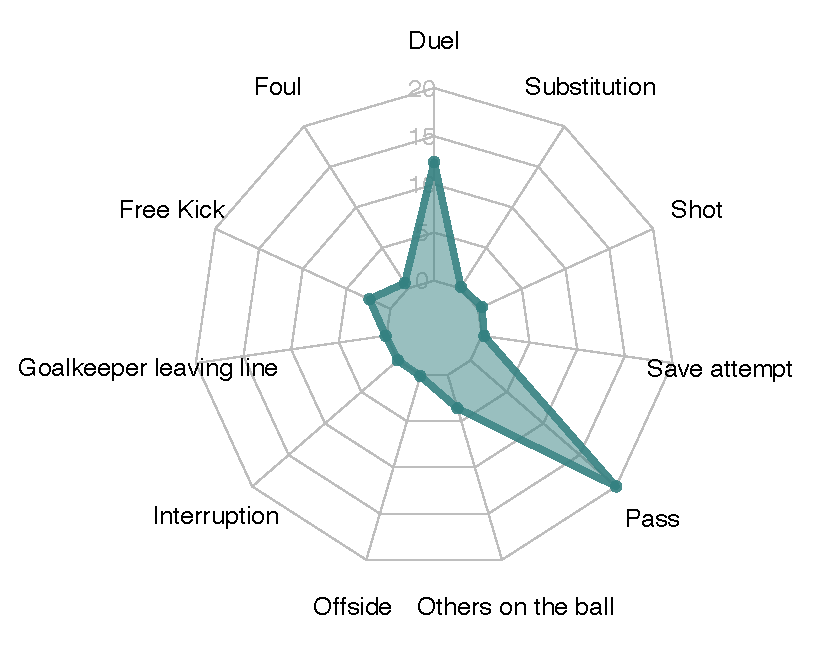
\includegraphics[scale=0.55]{F1_2fixed.pdf}
\caption{Donut Chart Figure and Radial Chart}\label{Radial Chart}
\end{center}
\end{figure}

From Figure \ref{Radial Chart}, it is evident that among all events, passes have the most significant portion. That also explains why it is necessary to deploy a good passing strategy in a game and to study the passing network to understand better what structure can be beneficial to the team performance. Figure \ref{Bar Plot of Passes per Game} shows how many passes made by all 30 players in each match. Some matches share some similar passing compositions, which indicates that along with teamwork, individual performance can also significantly affect the results of the game.

\begin{figure}[h!]
\begin{center}
\includegraphics[width=0.8\textwidth]{F2.pdf}
%fig2
\caption{Bar Plot of Passes per Game}\label{Bar Plot of Passes per Game}
\end{center}
\end{figure}

\subsection{Motif Analysis}
Motif Analysis is widely used to identify the patterns of passing network. In every network, the modules consist of different motifs, which plays a significant role in the performance of this network. A complex system cannot function properly unless it’s motifs and modules function properly.[1] In the past study, it showed that the analysis of the motif of players’ passing network could help pick strategies when facing different styles of opponents, contributing to scoring more goals to win the match[3].

\begin{figure}[h!]
\begin{center}
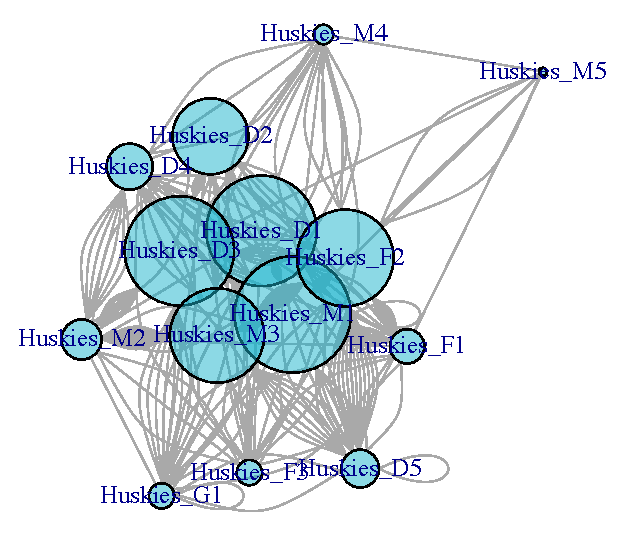
\includegraphics[width=.5\textwidth]{F3fixed.pdf}
%fig3
\caption{Passing Network of the First Match}
\end{center}
\end{figure}

In this paper, we will focus on the triadic configuration in every 38 matches. The triadic arrangement is a formation having three vertices, which is also can be seen as a 3-node motif. In all the 3-node cases, there are 2 undirected motifs and 13 undirected motifs[2]. 

\subsection {Scoring System of Motifs}
The aspects we are using to determine how well the motifs are doing, were found by taking using the scores and searching for the frequency and the last used motif related to that shot or score. 

We are using these aspect due to how versatile we believe we could make the scores and the shot events for weighing out the motif types. We manage to narrow down the motif types we would recommend to the coaches from 13 down to 2 by using this method. 

The scoring method we are using to weigh the motifs involved first taking a frequency of each motif in the match. We next multiply that value by the difference of the score for the game. This scales the score by the frequency of the motif so that we get an accurate idea on how beneficial or detrimental each motif was for the match. 

To balance out motifs that were more beneficial than others, a second metric is used besides the final score of the match and the frequency of the motif. The aspect we are using it the frequency of the motif resulting in a shot made against the opponent’s goal. This is then multiplied by the frequency of the motif in the entire game. This results in a balance of how much the model rewards wining in the game and how much the model punishes losing. We did not want the model to overly reward one aspect while overly punishing another aspect and after some basic experimenting we found a balance we thought worked the best. 
\begin{equation}
S_{Tj}= S_{Ej}+S_{Fj}=\sum_{i=1}^{38}{w_{ij}(S_{diff,j}+E_{ij})}
\end{equation}
From the dataset, we use R language to identify how many particular types of motifs appear in each match. Here we define an evaluation system to compare the frequency of motifs and also evaluate how frequently they are used to attempt to shot. The table 1 below shows the total weighted scores of the 13 motifs for the first 3 matches.

\begin{table}[thb]
\caption{Total Weighted Scores of 3-node Motifs}
\centering
\begin{tabular}{ c c c c c c c c c c c c c c}
\hline
Motif & 1&2&3&4&5&6&7&8&9&10&11&12&13\\
\hline
M 1 &.014& .045&.066&.014&.038&.031&.149&.319&0&.052&.045&.236&.156\\
%M 2&.05&0&0&0&0&0&0&0&0&0&0&0&0&\\
%\hline
M 2&-.027&-.153&-.24&-.053&-.073&-.067&-.28&-.127&-.027&-.16&-.087&-.42&-.26\\
\hline
\end{tabular}
\end{table}

\subsection{Clustering Analysis}
Cluster analysis is a class of techniques that are used to classify objects or cases into related groups called clusters. Based on the scores of each match for these 13 network motifs, we want to classify the games into several clusters depending on how “close” they are, which can show the similar passing patterns those matches share. After classifying both matches and motifs, we roughly can conclude that there are 3 clusters for both of them. The clustering results are as follows. 

\begin{equation}
d(x,y)=\sqrt{(x_1-y_1)^2+(x_2-y_2)^2+...+(x_n-y_n)^2}
\end{equation}
After classifying both matches and motifs, we roughly can conclude that there are 3 clusters for both of them. The clustering results are as follows.
\begin{table}[thb]
\caption{Cluster for Matches}
\begin{center}
\begin{tabular}{ c c c c}
\hline
Cluster& 1&2&3\\
\hline
Match &18,15,30,27,36,25,3&33,12,20,16,37,19,2,34,28&10,13,9,23,26,5\\
&5,6,17,31,11,1,14&21,7,32,29,22,38,3,4\\
Win: Tie: Loss&13:0:0&0:10:9&0:0:5\\
\hline
\end{tabular}
\end{center}
\end{table}

According to this Table 2, we can say that based on a specific motif pattern in the games, it does have some effect on the game results. The first cluster shows that by using a similar motif pattern, Huskies team tends to win a lot, and in the third cluster, they performed the worst, partly because they deploy a poor motif pattern. 

From Figure 4, the yellow color indicates positive and green color indicates negative, and the deepest the color is, the larger the absolute value of the score. Form clusters 1 and 3, we identify that both groups tend to use motif 12,13 the most. So, we cannot say that we should avoid or deploy motif 12 and 13 at this point. We need to consider a general case. To find out which motifs tend to work better in all the games, we compare the total scores of 38 matches to see which score the highest. Table 3 gives the overall weighted scores of 13 3-node motifs.

\begin{figure}[h!]
\begin{center}
\includegraphics[width=.6\textwidth]{F4.pdf}
\caption{Heat Map}
\end{center}
\end{figure}

\begin{table}[thb]
\caption{Total Weighted Scores of 3-node Motifs}
\begin{center}
\begin{tabular}{ c c c c c c c c}
%\nomargin
\hline
Motif & 1&2&3&4&5&6&7\\
Score &-0.372& 8.872&2.676&0.135&-0.360&-0.271&7.275\\
\hline
Motif &8&9&10&11&12&13\\
Score &-1.164&-0.210&-1.315&-0.749&-2.756&-1.372\\
\hline
\end{tabular}
\end{center}
\end{table}

 \begin{figure}[h!]
\begin{center}
\includegraphics[width=.45\textwidth]{F5.pdf}
\caption{Motif Scores}
\end{center}
\end{figure}

\begin{figure}[h!]
\begin{center}
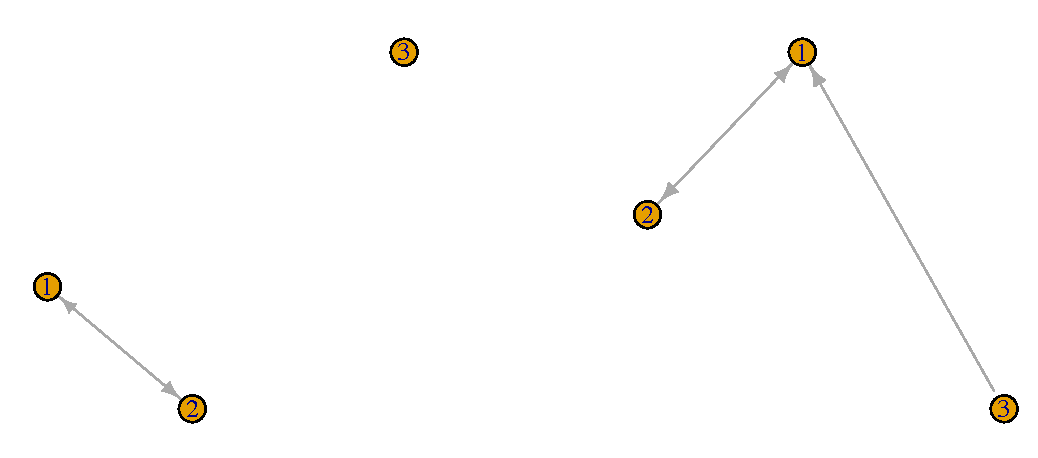
\includegraphics[width=.4\textwidth]{F6_1f.pdf}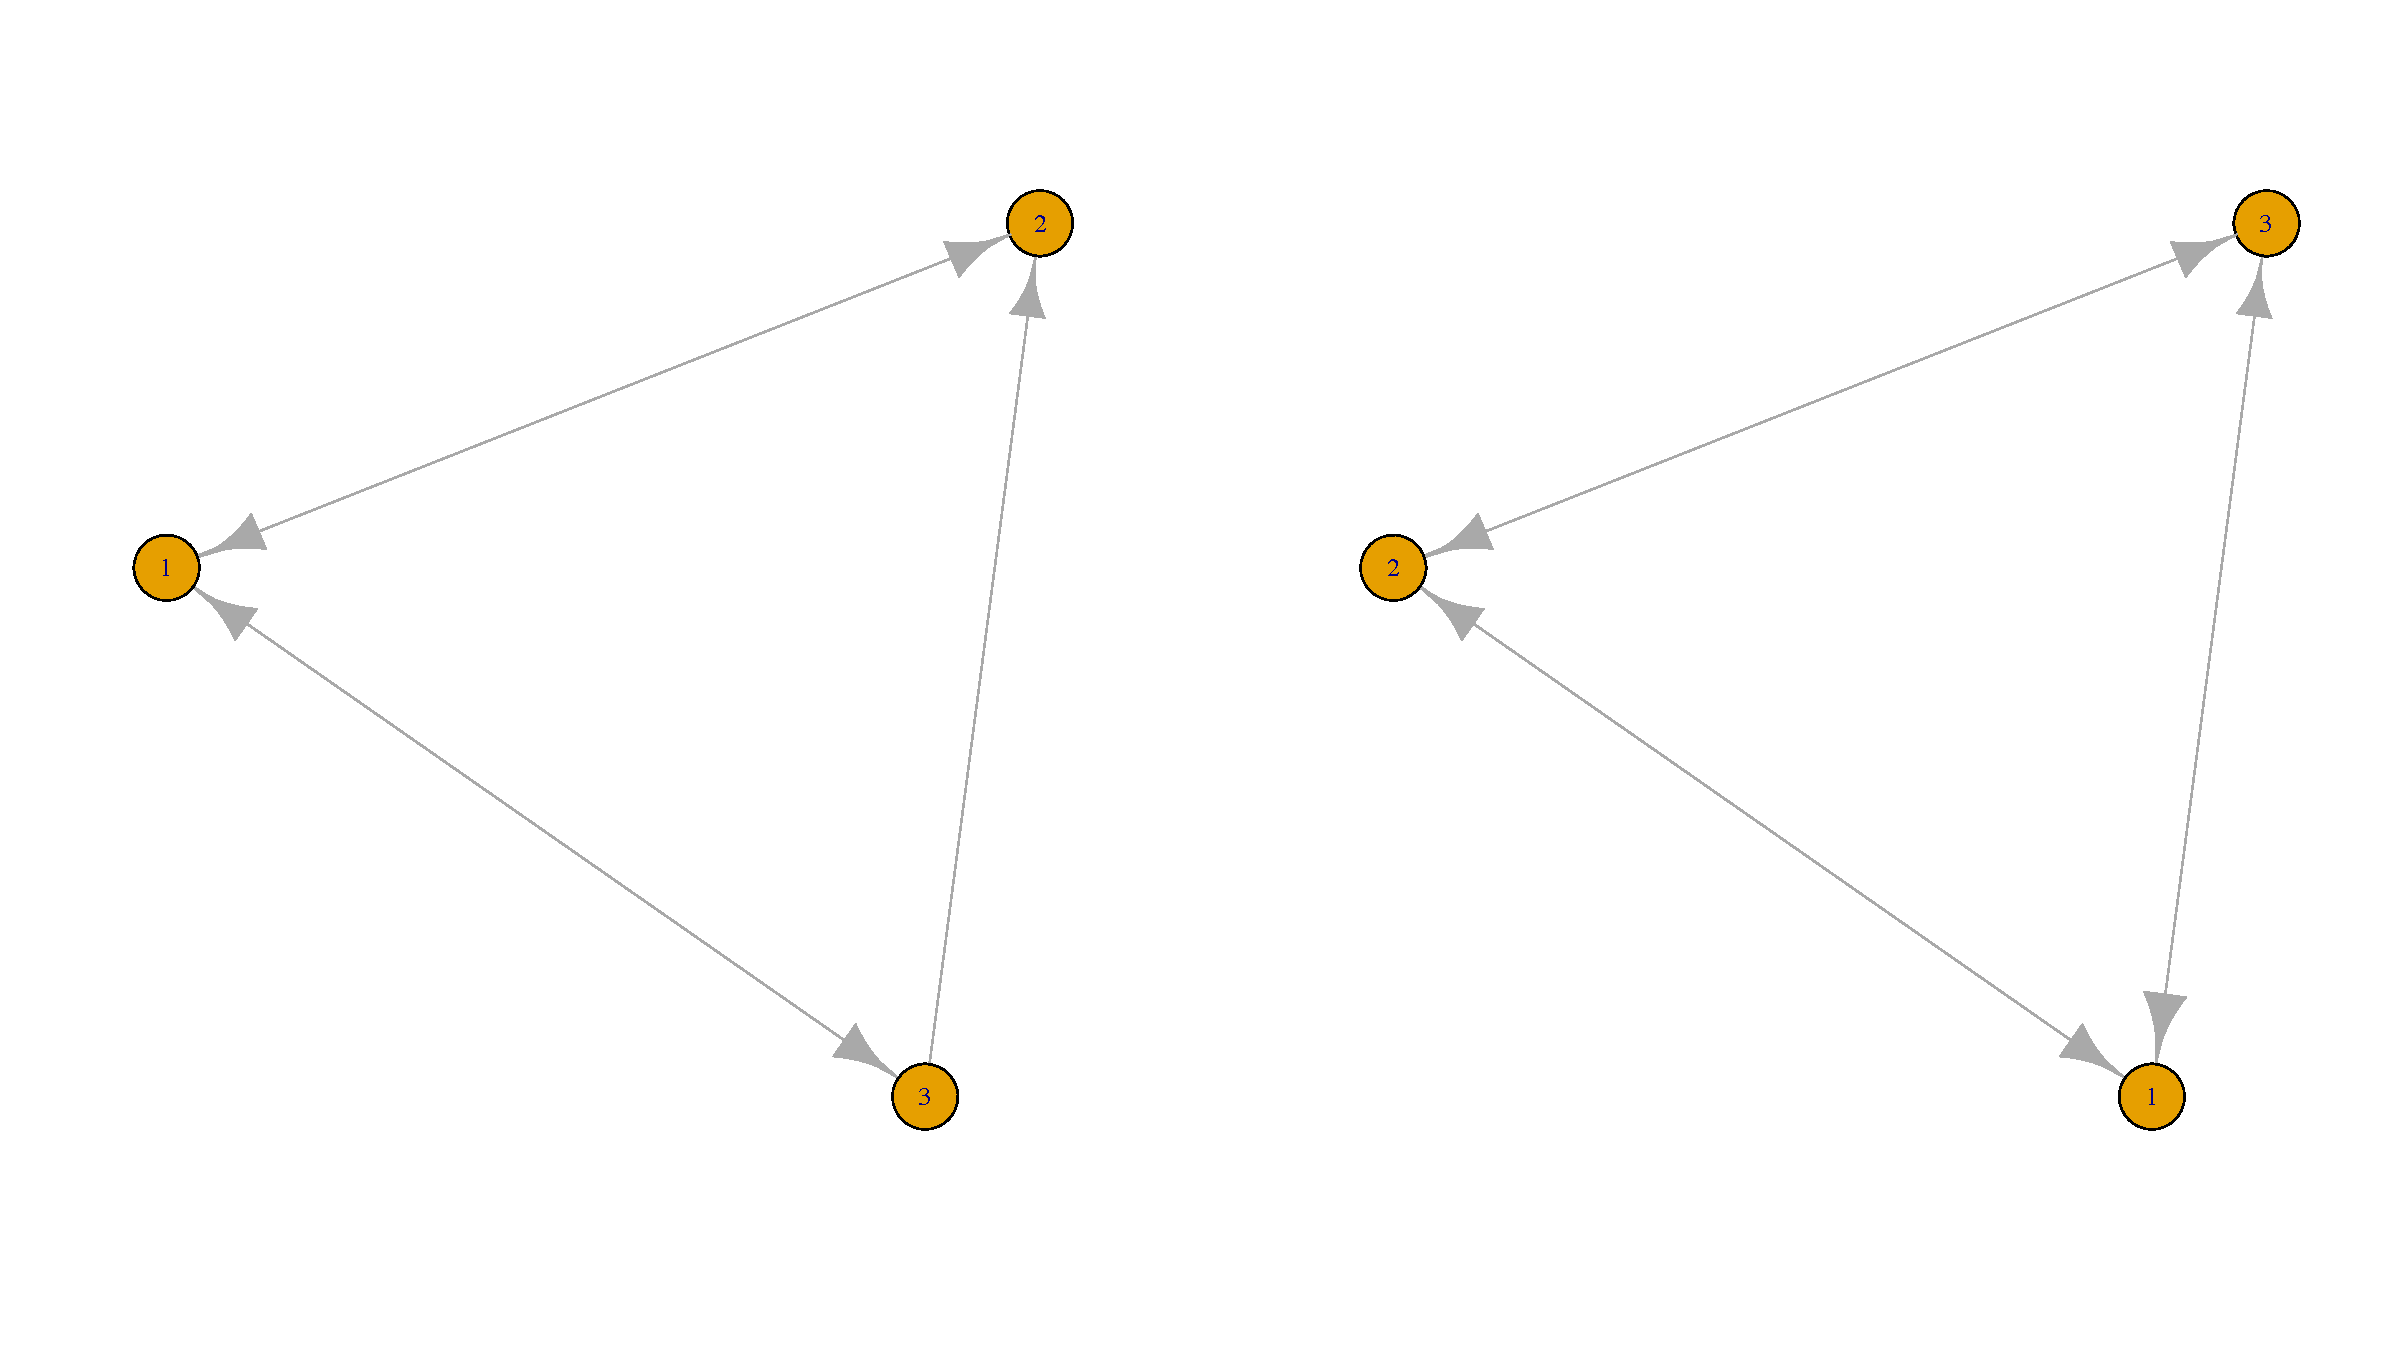
\includegraphics[width=.4\textwidth]{F62.pdf}
\caption{Motif 1,3,12,\&13}
\end{center}
\end{figure}

 From Figure 5, we can clearly see that motif 1, 3 have the highest score, while motifs 12, 13, and 10have the lowest score. With the discussion before, we may say deploying motifs 12 and 13 would be risky strategies, which make it more possible to score a goal or lose the ball. However, using motif 1 and motif 3 ,7 is suggestive to make a successful pass and therefore contribute to scoring a goal. See Figure 6.
 


\newpage

\section{Performance Prediction}
\subsection {Indicators of Performance}

With the development of technology, there are many ways for football experts to get statistics during games to monitor individual performance. However, it is unclear how team processes lead to greater performance or how individual roles and strengths are combined for optimal results.[2] Due to the low scores and uninterrupted flow of the ball, it is somehow more challenging to analyze football quantitatively than other sports. However, ideas of data-mining technology and machine learning give us great insight. Based on the network model for each match, we can extract some features as a performance indicator to measure different facets of teamwork, such as configurational and dynamical aspects.  Here we propose 9 indicators, which are: $\Delta_x, \Delta_y,\lambda,\mu_{pass},\mu_{dis},\sigma_{pass},\sigma_{dis},\omega,$ and $P_{Ti},$ with the motifs pattern, which reflects the structural aspect, to evaluate the overall performance of team play 1378. (Figure 7 Review of Indicators).

\begin{figure}[h!]
\begin{center}
\includegraphics[width=.6\textwidth]{F7.png}
\caption{Review of Indicators}
\end{center}
\end{figure}

\subsection{Extract Indicators}
Let the Huskies team as an example, we will show some statistics of the indictors extracted form 38 matches. From Figure 8, we can see that among 9 indicators, some of them are highly correlated, such as average passes, the variance of the passes of the player in a match, total passes, and the largest eigenvalue. By definition, the average should be independent on the variance, so the result here shows that in a football game, if the team tends to scores many goals, it is likely that one of the players contributes the most and make a discrepancy among his/her teammate. It is not surprising that centroid x and y are slightly correlated with other indicators, almost independent from others. In addition, there is not a highly negative correlation among all the indicators.


From Figure 9, it shows the average passes and average distance concerning every 38 matches. The error is the standard deviation of 38 value, which shows that among different matches, the average passes fluctuate, while the average distance of passes between matches tends to be more stable, which comes with a smaller error. 

\begin{figure}[h!]
\begin{center}
\includegraphics[width=.45\textwidth]{F8f.pdf}
\caption{Correlation Plot of Indicators}
\end{center}
\end{figure}

\begin{figure}[h!]
\begin{center}
\includegraphics[width=.4\textwidth]{F9_1.pdf}\includegraphics[width=.4\textwidth]{F9_2.pdf}
\caption{Average passes with Error Plot and Average Distance with Error}
\end{center}
\end{figure}
\begin{figure}[h!]
\begin{center}
\includegraphics[scale=0.4]{F10_1.pdf}\includegraphics[scale=0.4]{F10_2.pdf}
\caption{Coordinate of Centroid (x,y) and Eigenvalue for 38 matches}
\end{center}
\end{figure}

From Figure 10 left, we can have an intuitive impression on where the centroid of different passes network for each game located.  The distribution of x, y appears to be right-skewed, and the interquartile range is around 5. From Figure 10 right, we can see the largest eigenvalue of the adjacency matrix of each network, which measures the 
network strength.[3] As a rule of thumb, networks with a higher number of links (passes) will have a higher $\lambda_1$ and networks with the important nodes connected between them (known as assortative networks) will also have higher $\lambda_1$ than networks where the hubs (i.e., important players) are not directly connected between them. [4]

\subsection{Prediction Comparison}
Based on the history of 38 past games and the indicator of team Huskies, we use several machine learning methods to create a classification model. We define the result of games “win”, “tie”, “loss” as {1,0,-1}.  Since we only have 38 samples, which is considered small. We use 10-fold cross-validation, that is every time we sample 30 matches as training data, and the rest 8 matches as testing data. By taking the mean of the error rate as estimated error rate, then we can get the estimated accuracy of each classifier.

\begin{table}[thb]
\caption{Accuracy of Prediction of Huskies Team}
\begin{center}
\begin{tabular}{ c c}
\hline
Classifier&Estimated Accuracy\\
\hline
Logistic Regression& 57.89\%\\
LDA&75.32\%\\
SVM&92.11\%\\
Random Forest & 65.34\%\\
Naive Bayes & 76.31\%\\
\hline
\end{tabular}
\end{center}
\end{table}
Among these three classifiers, Support Vector Machine has classification accuracy of about 92.11\%, so it is considered to be the best model to predict the game results. And the performance indicators seem to be useful to determine the success of teamwork.

\subsection{Verification}
In order to verify the effectiveness and usefulness of our performance data, we attain the values of all indicators of opponent team to verify if we use these features and certain classifier, we still be able to have an accurate model to predict the results. With 38 matches and 19 opponent’s and Huskies’s information, we are able to expand our sample size. After 10-fold cross validation, the estimated accuracy table is as follows.
\begin{table}[thb]
\caption{Estimated Accuracy Modifiers}
\begin{center}
\begin{tabular}{ c c }
\hline
Classifier&Estimated Accuracy\\
\hline
Logistic Regression& 59.02\%\\
LDA&71.53\%\\
SVM&77.38\%\\
Random Forest &82.46\%\\
Naive Bayes & 73.82\%\\
\hline
\end{tabular}
\end{center}
\end{table}
\begin{figure}[h!]
\begin{center}
\includegraphics[width=.6\textwidth]{F10_3.pdf}
\caption{Important Score of Indicators}
\end{center}
\end{figure}
In this case, the Random Forest has the highest classification accuracy at 82.46\%. From the Fig 11, we can tell that among 9 factors, centroid (x, y), total passes, standard deviation and average of pass distance and eigenvalue consider are considered to be the 5 most significant factor while doing prediction. While whether side or the average passes are trivial, which can be interrelated as that whether play the game at home or away have little to do with the results of the game. And rather than have a higher average pass, if the MVP (Most Valuable Player) makes more accurate passes and shots more than others, with a good passing network, we still can expect the success for the whole team.



\section{Insights to Coach}
There are three aspects for the coach to make an improvement with for the next season.
\subsection{Passing Strategy}
From the Motifs identification and Clustering analysis, we can see that when Huskies won the games in the last season, all 13 of them appeared to show a homogenous distribution of motifs frequencies. This kind of distribution shows generally high motifs frequency of both complex 3-node motifs (more than three edges) and both simple 3-node motifs (no more than three edges). The higher the frequencies of motifs reveal the higher the total passes. In a sense, the more the passes, the more likely to score and to win the game. However, the complex motifs 12 and 13 are both used a lot not matter the Huskies won or lost. That means too complex passing network might be tackled by opponent and break the pass. So, to properly use complex passing motifs combine with simple 3-node motifs may optimal the results, and it should be general strategies.
\subsection{Configuration}
The centroid of a network is one of the measurements to demonstrate the type of configuration. If the coordinate of centroid is closer to opponent’s goal area, then is an offending configuration; otherwise, if the coordinate is closer to own goal area, then it is defending configuration. Since in the section 3.4, we verify that centroid($x,y$) is a significant factor contributing to winning, it is very important for coach and the players to make adjustment according to the situation at each timing of the game, which requires players adaptability and flexibility. For example, the Huskies first offend and score 3-0, then the rest of the time they should keep defending. Coaches should focus on training the players to quickly adapt to several configurational transformations to come up with better strategy when having different score difference during a game.
\subsection{Individual Dynamic}
There are four indicators to measure the dynamic of players on field. The distance and the number of pass are two aspects to indicate a player’s performance: strength and agility. From section 3.2, the average distance of players of all 38 games does not show too many variations, however the number of average passes do. While total passes weighted more than average passes in predicting success, that is to say the teamwork of the whole teams are more important than individual performance. We suggest that the players should keep moving around the field to make more interaction with teammates, especially to help the striker, will certainly helpful to improve the team success.
\section{Applications}

\subsection{Purpose of Applications}
	The purpose of this kind of application is less to do with actual advice on how to utilize teamwork, but rather to create a way of analyzing the network and the data in such a way as to make solutions that work for that specific problem. For instance, it may be possible that a motif that works well for moving a football ball towards the goal and past an opposing team member, will not work well for transferring ideas back and froth between team members.
\subsection{Non Sport Applications}
	The applications of teamwork analysis do not need to be limited to just analysis of sports, board games, and video-games. There is already a president of all sorts of models being repurposed from sports and other games into general models of cooperation and teamwork. While it is not necessary that the model applies to every type of cooperative team, it is necessary that it can be applied to the majority of them.[2]

	The passing network’s motifs are able to model the dynamic way that teams interact on a micro scale. By only focusing on three team members at a time it is possible to give feedback on that specific type of interaction. By finding which motifs are being used throughout the team it is possible to compare it to the results of the passing network’s optimal motifs and then adjust the team accordingly[1]. 
\subsection{Applications in Practice}
	In practice the motifs for the teamwork network would be much implemented in a much easier way than the motifs in the middle of a football match. This is because unlike in a football match, a normal operating team can take a moment and consider their next move. In this way the team can think back on which motifs are the best to use and act accordingly. This may be to always hand off your portion of the project to another team member who will in turn transfer it over to another team member. Or it could wrap around back to the original person who started the motif. 
	The purpose of this kind of application is less to do with actual advice on how to utilize teamwork, but rather to create a way of analyzing the network and the data in such a way as to make solutions that work for that specific problem.[8] 

%\section{Evaluation of the Model}
%\subsection{Network Motif Analysis}
%There are four indicators to measure the dynamic of players on field. The distance and the number of pass are two aspects to indicate a player’s performance: strength and agility. From section 3.2, the average distance of players of all 38 games do not show too many variations, however the number of average passes do. While total passes weighted more than average passes in predicting success, that is to say the teamwork of the whole teams are more important than individual performance. We suggest that the players should keep moving around the field to make more interaction with teammates, especially to help the striker, will certainly helpful to improve the team success.
%\subsection{Performance Indicator}
%In the section, we extract 9 indicators (features) to reflect performance of teamwork. These 9 indicators mainly measure the configuration of network and dynamical of the team members, which makes it possible to quantify the performance of the whole teamwork and network as well. Based on the 9 indicators, it is verified that by using suitable machine learning methods, over 50\% of the match results can be correctly classified. When we restrict the data scale for Huskies team, the estimated accuracy can be raised to 92\% by SVM (Support Vector Machine). For a wider scale, the Random Forest performance the best to predict the results for all opponents and Huskies with 82.46\%. Therefore, these 9 performance indicators are reasonable to use for evaluate the performance of teamwork for generally. If the sample size is expanded to train the model, we may find another classifier works better. So it has yet to figure out an unique combination of these indicators to evaluate teamwork in a general case.
\section{Conclusion}

In the Network Motif Analysis section, we look at the passing network between players of Huskies and to identify the frequencies of 13 directed 3-node motifs of each match. Instead of studying the complex structure of network, it is more effective to break down the outframe and focus on the modules. Based on a micro pattern, we weigh each motifs of the match according to the score and shots and cluster past football event for Huskies team based on the motifs score. From the scoring system we propose, we can decide which motifs pattern is suggested and give the coach some insight on the passing network. However, we do not take distance of each passes, individual players’ location into account in this step, which may help explain the macro aspect of the passing network.

In the Performance Indicator system, we extract 9 indicators (features) to reflect performance of teamwork. These 9 indicators mainly measure the configuration of network and dynamical of the team members, which makes it possible to quantify the performance of the whole teamwork and network as well. Based on the 9 indicators, it is verified that by using suitable machine learning methods, over 50\% of the match results can be correctly classified. When we restrict the data scale for Huskies team, the estimated accuracy can be raised to 92\% by SVM (Support Vector Machine). For a wider scale, the Random Forest performance the best to predict the results for all opponents and Huskies with 82.46\%. Therefore, these 9 performance indicators are reasonable to use for evaluate the performance of teamwork for generally. If the sample size is expanded to train the model, we may find another classifier works better. So, it has yet to figure out a unique combination of these indicators to evaluate teamwork in a general case.

%%%%%%%%%%%%%%%%%%%%%%%%%%%%%%
%%% ---------------
\begin{thebibliography}{9}


\bibitem{Cintia} 
Cintia, Paolo, et al. "The harsh rule of the goals: Data-driven performance indicators for football teams." \textit{2015 IEEE International Conference on Data Science and Advanced Analytics (DSAA)}. IEEE, 2015.

\bibitem{Buldu} 
Buldú, J. M. et al. “Defining a Historic Football Team: Using Network Science to Analyze Guardiola’s F.C. Barcelona.” \textit{Scientific Reports 9.1 (2019)}: n. pag. Crossref. Web.

\bibitem{Duch} 
Duch, Jordi, Joshua S. Waitzman, and Luís A. Nunes Amaral. "Quantifying the performance of individual players in a team activity." \textit{PloS one} 5.6 (2010).

\bibitem{Gursakal}
GÜRSAKAL, N , YILMAZ, F , ÇOBANOĞLU, H , ÇAĞLIYOR, S . "Network Motifs in Football". Turkish Journal of Sport and Exercise 20 (2018 ): 263-272 <https://dergipark.org.tr/en/pub/tsed/issue/40371/465664>

\bibitem{Bekkers}
Bekkers, Joris, and Shaunak Dabadghao. "Flow Motifs in football: What can passing behavior tell us?." \textit{Journal of Sports Analytics Preprint} (2017): 1-13.

\bibitem{Park}
K. Park and A. Yilmaz, "Social Network Approach to Analysis of football Game," \textit{2010 20th International Conference on Pattern Recognition}, Istanbul, 2010, pp. 3935-3938.

\bibitem{Gyarmati}
Gyarmati, Laszlo, Haewoon Kwak, and Pablo Rodriguez. "Searching for a unique style in football." \textit{arXiv preprint arXiv:1409.0308} (2014).

\bibitem{Celemente}
Clemente, Filipe Manuel, et al. "General network analysis of national football teams in FIFA World Cup 2014." \textit{International Journal of Performance Analysis in Sport 15.1 }(2015): 80-96.

\bibitem{Pena}
Pena, Javier López, and Hugo Touchette. "A network theory analysis of football strategies." \textit{arXiv preprint arXiv:1206.6904 }(2012).

\bibitem{Cotta}
Cotta, Carlos, et al. "A network analysis of the 2010 FIFA world cup champion team play." \textit{Journal of Systems Science and Complexity 26.1 (2013): 21-42.}

\bibitem{Aguirre}
Aguirre, J., Papo, D. \& Buldu, J. M. Successful strategies for competing networks. Nat. Phys. 9, 230 (2013). 

\end{thebibliography}

\end{document}










%\begin{appendices}
%\section{Matlab Code}\label{Matlab Code}
%
%Here are simulation programmes we used in our model as follow.\\
%
%\textbf{\textcolor[rgb]{0.98,0.00,0.00}{Input matlab source:}}
%\lstinputlisting[language=Matlab]{./code/test.m}
%\lstinputlisting[language=Matlab]{./code/geoCode.m}
%\lstinputlisting[language=Matlab]{./code/geoDist.m}
%\lstinputlisting[language=Matlab]{./code/createfigure.m}
%
%
%
%
%\section{R Code}\label{R Code}
%
%Here are simulation programmes we used in our model as follow.\\
%
%\textcolor[rgb]{0.98,0.00,0.00}{\textbf{Input R source:}}
%\lstinputlisting[language=R]{./code/Lassotest.R}
%
%\end{appendices}
\end{document}

%%
%% This work consists of these files mcmthesis.dtx,
%%                                   figures/ and
%%                                   code/,
%% and the derived files             mcmthesis.cls,
%%                                   mcmthesis-demo.tex,
%%                                   README,
%%                                   LICENSE,
%%                                   mcmthesis.pdf and
%%                                   mcmthesis-demo.pdf.
%%
%% End of file `mcmthesis-demo.tex'.
